\chapter{Materiales y Métodos}
\section{Materiales}
\subsection{Datos públicos} 
Para este TFG se ha utilizado diversos conjuntos de datos públicos para la 
evaluación y elección de los modelos anteriormente descritos. De entre ellos 
están SJTU\cite{SJTU}, WPC\cite{WPC1,WPC2} y LS-SJTU-PCQA\cite{ResSCNN}.

El primer de ellos, parate de 10 nubes de puntos de referencia, ver Figura \ref{fig:SJTU}, 
a las cuales se aplican 7 tipos de distorsiones. Estas son: compresión, ruido 
al color, ruido geométrico, ruido gaussiano y combinación entre ellas, ver Tabla \ref{tab:SJTU}. Todas se aplican en una escala creciente
de intensidad del 1 al 6. Luego, se obtiene un MOS de 10 individuos para las 420 
nubes de puntos. 

\begin{figure}[htp]
  \centering 
    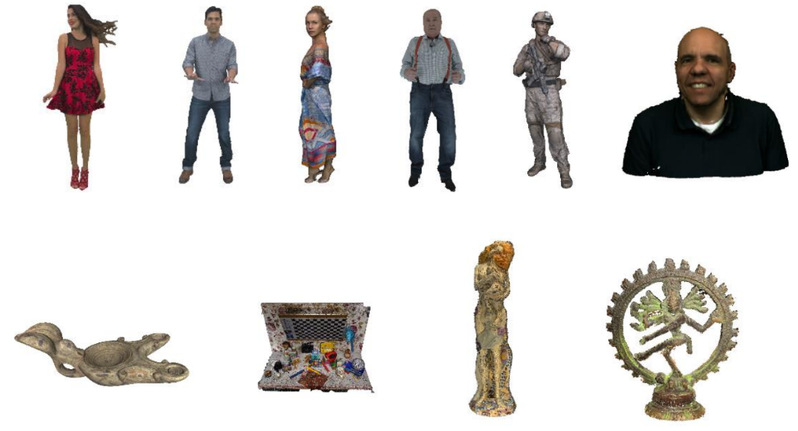
\includegraphics[width=0.95\textwidth]{imagenes/chapter4/SJTU}
    \caption{Ejemplo de conjuntos de datos SJTU\cite{SJTU}.}
    \label{fig:SJTU}
\end{figure}

\begin{table}[htp]
  \centering 
  \scriptsize
  \begin{tabular}{|c|c|}
    \hline
    Número & Tipo de Distorsión \\ 
    \hline 
    0 & OT: Compresión octree\cite{OctreeCompression} \\ 
    \hline 
    1 & CN: Ruido fotométrico\\ 
    \hline 
    2 & DS: Submuestreo uniforme \\
    \hline 
    3 & DS + CN \\
    \hline 
    4 & DS + GGN \\
    \hline 
    5 & GGN: Ruido geométrico gaussiano \\
    \hline 
    6 & CN + GGN \\ 
    \hline 
  \end{tabular}
  \caption{Ejemplo de distorsiones en SJTU\cite{SJTU}.}
  \label{tab:SJTU}
\end{table}

El segundo, WPC\cite{WPC1, WPC2}, también posee distorsiones como submuestreo uniforme y 
ruido gaussiano (aplicados de manera distinta), pero a su vez posee nuevos tipos 
de distorsiones. Estos son basados en distintos tipos de compresión: V-PCC, G-PCC y \emph{trisoup}.
Además, posee distintos modelos de nubes de puntos, ver Figura \ref{fig:WPC}, que 
pueden influir en el rendimiento del modelo si no es lo suficientemente amplio 
y representativo de lo que puede encontrarse. 

\begin{figure}[htp]
  \begin{center}
    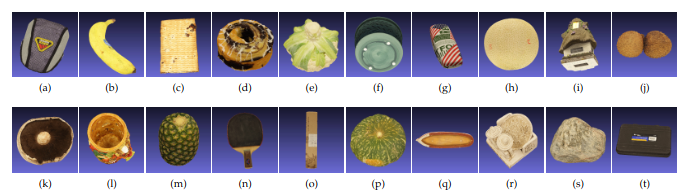
\includegraphics[width=0.95\textwidth]{imagenes/chapter4/WPC}
  \end{center}
  \caption{Ejemplo de conjunto de datos WPC\cite{WPC1, WPC2}.}
  \label{fig:WPC}
\end{figure}

Los dos anteriores han sido utilizados sobre todo para la evaluación y elección 
del modelo de inferencia a utilizar. Son los conjuntos de datos más conocidos 
y que habitualmente están presentes en las publicaciones. Además, se realizaron 
pruebas de ejecuciones de los métodos de código abierto para verificar los 
resultados. Todos estaban dentro de un margen de error aceptable.

Sin embargo, el último es el que finalmente se utiliza para entrenar un modelo para estimar 
la calidad de las imágenes médicas. Esto es porque es el mayor conjunto de datos, 
en el momento de escritura, y posee tipos de distorsiones que pueden simular 
lo que sería ciertos errores y ruidos presentes en imágenes médicas. Por ejemplo, 
el ruido gaussiano (simular errores de transmisión y almacenado de datos), 
rotación y movimiento local (simular el movimiento del paciente) y compresión 
octree y por submuestreo uniforme (algoritmos de compresión comúnmente usados).
Aparte, es el con mayor amplitud de modelos base, con distintos tipos y categorias 
de objetos, ver Figura \ref{fig:LS-SJTU-PCQA}.

\begin{figure}
  \begin{center}
    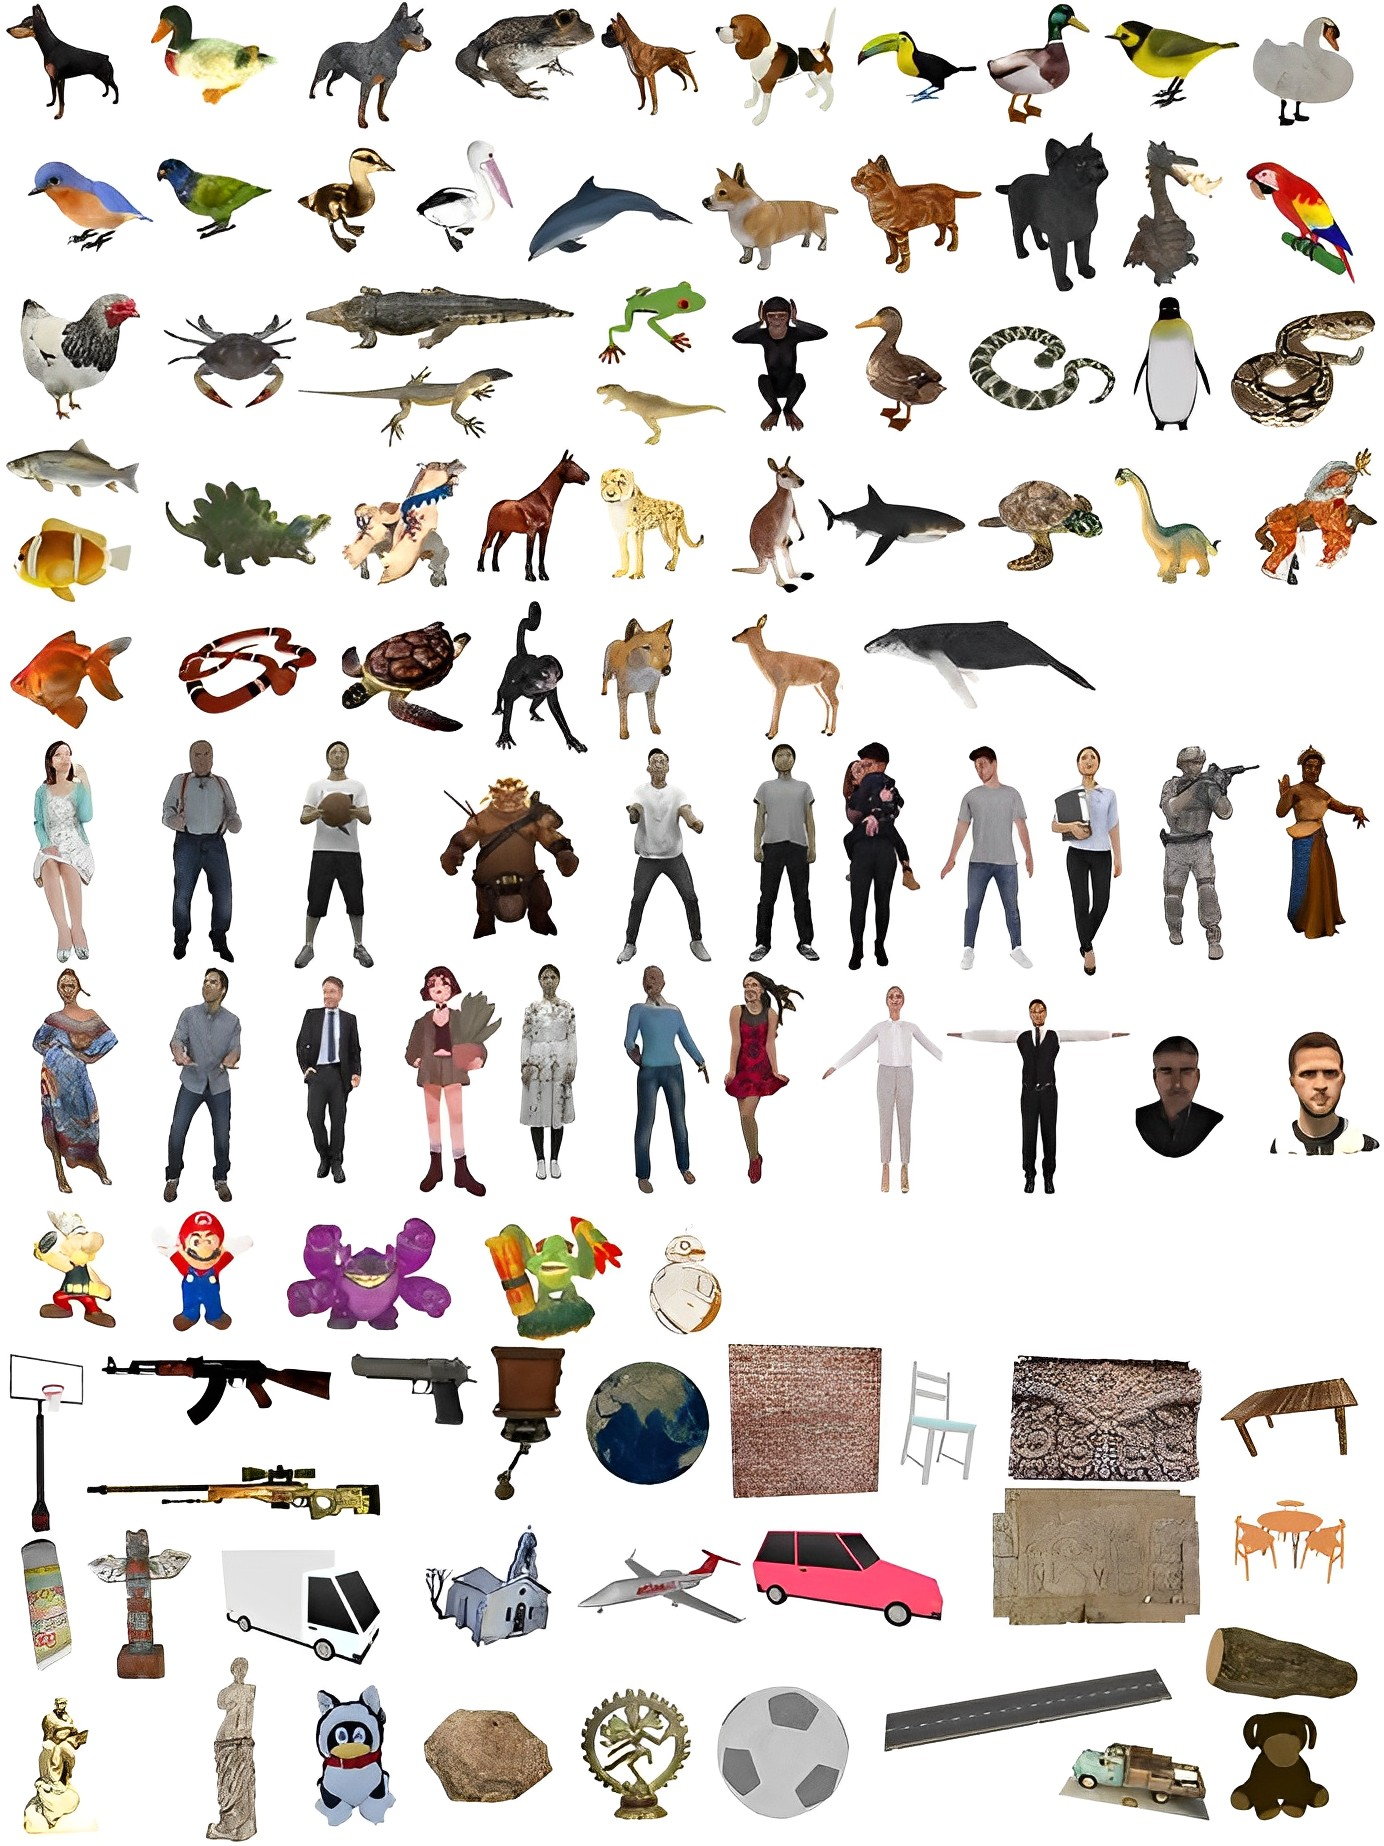
\includegraphics[width=0.95\textwidth]{imagenes/chapter4/LSPCQA}
  \end{center}
  \caption{Ejemplo de conjunto de datos LS-SJTU-PCQA\cite{ResSCNN}.}
  \label{fig:LS-SJTU-PCQA}
\end{figure}

\subsection{Conjunto de datos médicos}
\label{sec:OurData}
Para este TFG se tiene disponible una colección 26 directorios DICOM, de distintas
partes del cuerpo, de 2 distintos individuos. 
De los cuales han sido segmentados las clavículas, el seno frontal y el seno Maxilar. 
A parte, disponemoss de volúmenes del cráneo de otros 3 individous, una pubis izquierda y
una pubis derecha, ver Figura \ref{fig:OurDataExample}. Es decir, en total dispones de 11 nubes de puntos de alta 
calidad, que representan distintos volúmenes de exámenes médicos.

\begin{figure}[htp]
  \begin{subfigure}[b]{0.49\textwidth}
  \centering 
  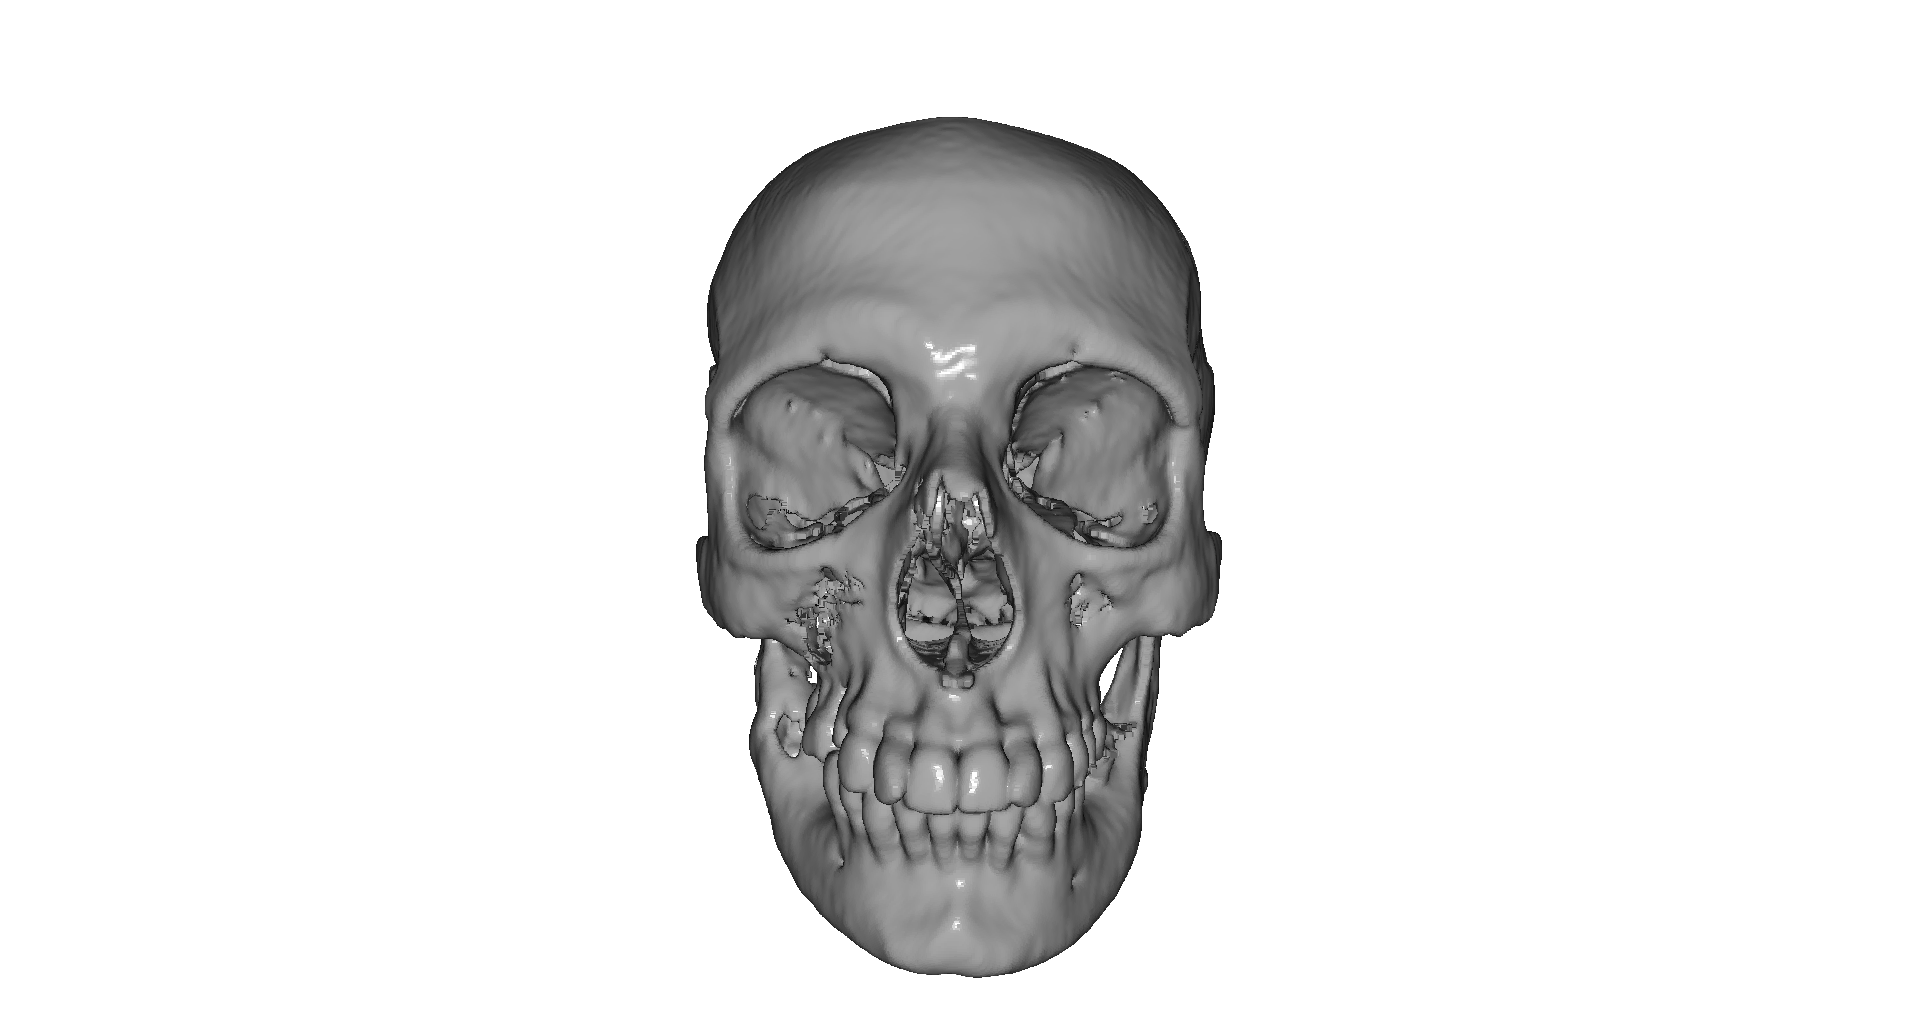
\includegraphics[width=\textwidth]{imagenes/chapter4/Craneo12018377.png}
  \end{subfigure}
  \begin{subfigure}[b]{0.49\textwidth}
  \centering 
  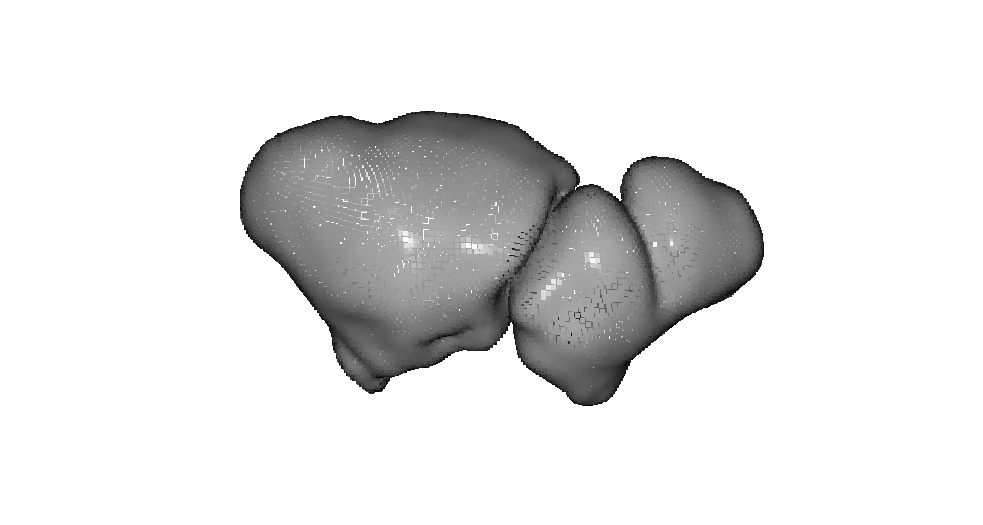
\includegraphics[width=\textwidth]{imagenes/chapter4/SenoFrontal100205.png}
  \end{subfigure}

  \begin{subfigure}[b]{0.49\textwidth}
  \centering 
  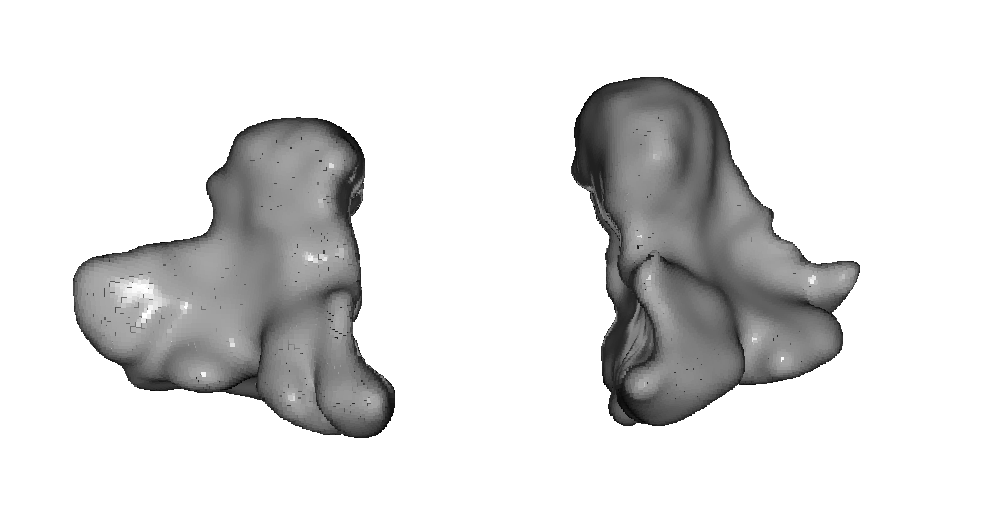
\includegraphics[width=\textwidth]{imagenes/chapter4/Maxilar100205.png}
  \end{subfigure}
  \begin{subfigure}[b]{0.49\textwidth}
  \centering 
  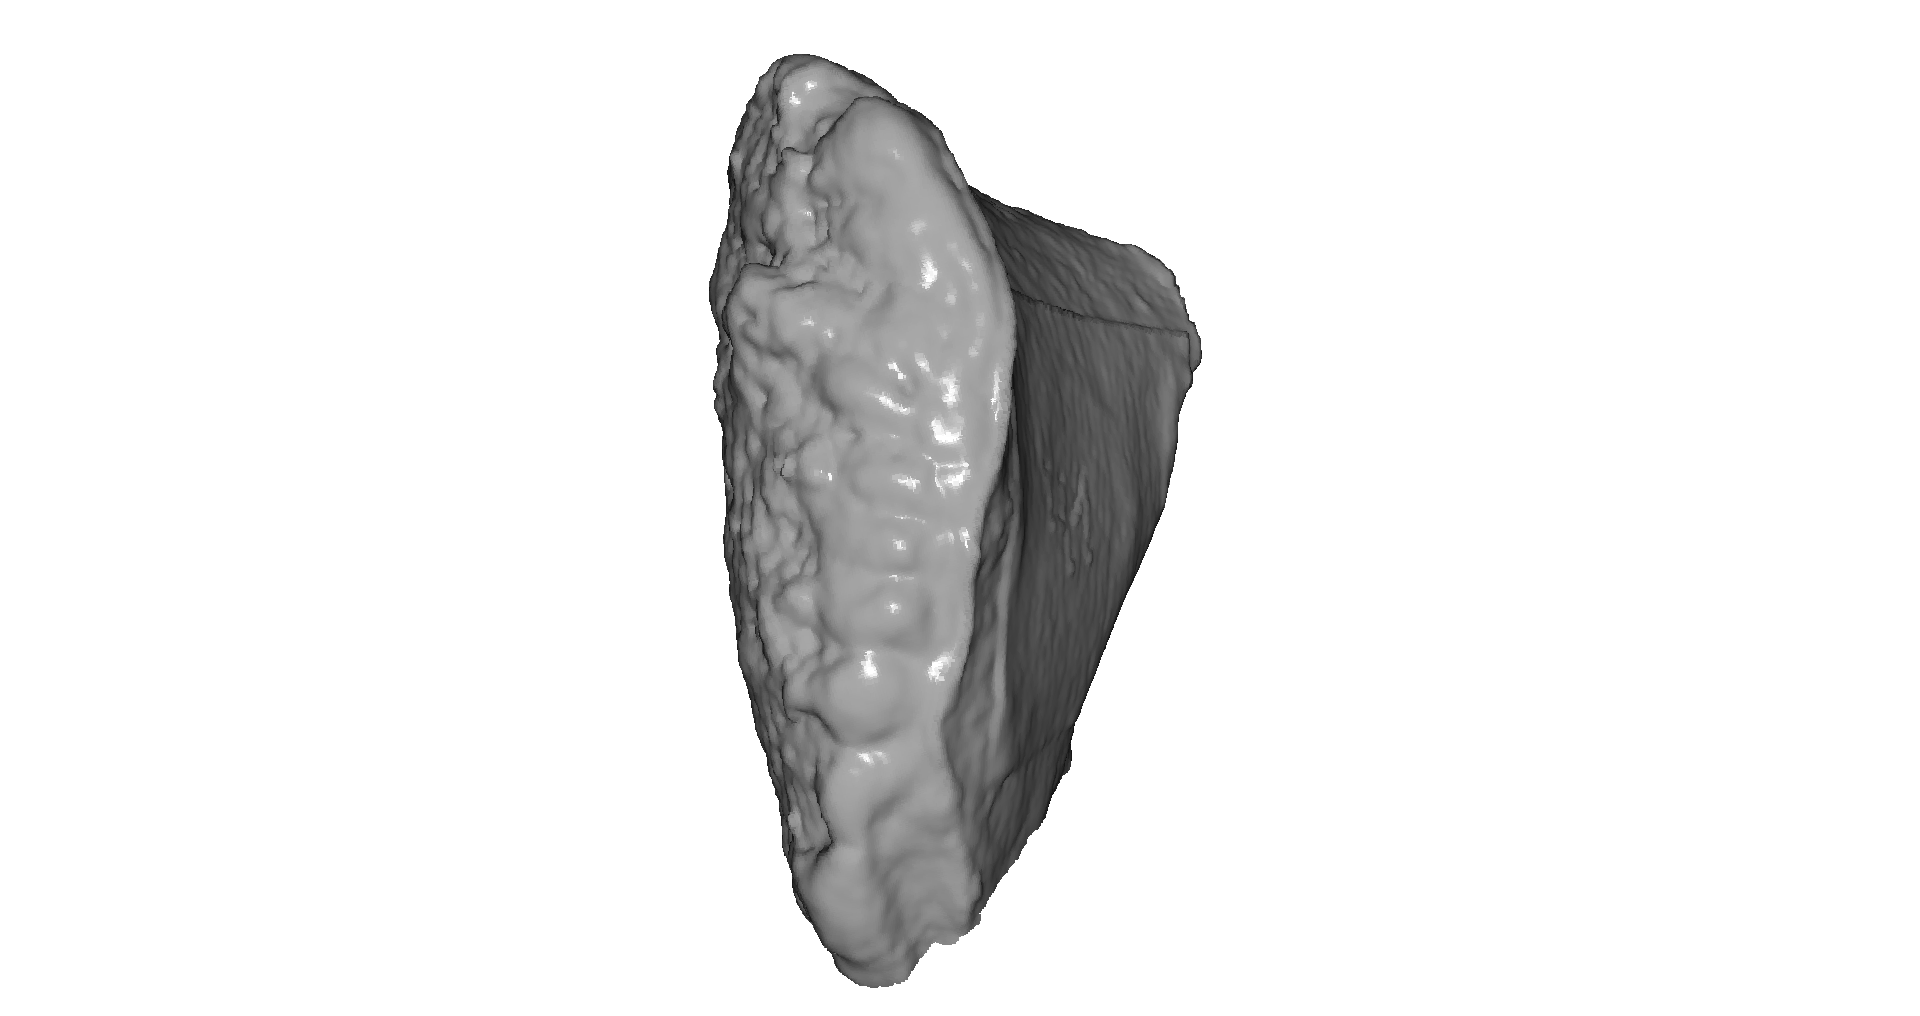
\includegraphics[width=\textwidth]{imagenes/chapter4/PubisDch.png}
  \end{subfigure}
  \caption[Ejemplo de nuestras imágenes médicas]{Ejemplo de nuestras imágenes médicas.
  Arriba a la izquierda tenemos un cráneo y a su derecha un seno frontal. 
  Abajo a la izquierda tenemos un maxilar y a su derecha el pubis derecho.}
  \label{fig:OurDataExample}
\end{figure}

A estos datos no se hicieron ningún tipo de pre-procesado, apenas se centraron 
las nubes de puntos a los ejes (operación necesaria para hacer la rotación para 
las distintas perspectivas, más detalles en la sección \ref{sec:Implementacion})
y se eliminaron aquellos puntos aislado de todos, frutos de errores en el 
algoritmo de generación de las nubes de puntos a partir de segmentaciones DICOM.

\section{Métodos}
Como se pudo observar en la Sección \ref{sec:EstadoDelArte}, actualmente hay una 
tendencia, justificada, a los métodos de aprendizaje profundo. Además, se tuvo 
que descartar todos los métodos que tuvieran en cuenta información de textura, 
cosa que no existe en los volúmenes médicos habituales. Además, necesitamos 
información perceptual de la imagen en su totalidad y no de regiones locales 
específicas. Es por ello, que optamos por evaluar el método VQA\cite{VQA-PC}.

\Brian[{Debería añadir un apartado sobre el método de NSS que probamos?}]{Como hice la 
  prueba de ejecución del método Zhang et al\cite{NR3DQA}, me pregunto si debería 
dedicar un apartado de métodos a ello para justificar aún más el método ML VQA-PC. 
Para ello imagino que quedaría pendiente una prueba de ejecución sobre LS-SJTU-PCQA, 
pero a priori, gracias al código abierto pude replicar el paper con los datos de SJTU. 
Luego probé utilizar algunas métricas más de los valores singulares que se suelen utilizar 
en segmentación y obtuve algunos resultados mejores en SJTU. En seguida probé 
con las imágenes médicas, pero obtuve 0.24.
}
\subsection{VQA-PC}
Zhang et al\cite{VQA-PC} propusó un modelo de estimación de calidad de nubes 
de puntos utilizando proyecciones 2D de diferentes perspectivas. 
Observaron que los métodos que trabajan directamente sobre la nube de puntos tienen
una elevada dificultad computacional, sin suponer una mejora excesiva, y que 
deben todavía que madurar en el campo dado la alta complejidad de las nubes de puntos.
Por ello proponen utilizar proyección multi-vista. No obstante, argumentó que 
los métodos anteriores de proyección se basan en la hipótesis de que los humanos 
percebimos la calidad de modelos 3D desde una perspectiva estática, cosa que no 
es cierta en la práctica dado que los objetos 3D permiten operaciones geométricas 
de rotación y escalado.
Y por ello, proponen unificar la percepción estática con la dinámica tratando 
a las proyecciones como videos.

De esta forma, se puede extraer características espaciales y temporales, como 
discutido en la Sección \ref{sec:VideoCNN}, utilizando redes convolucionales 
adaptadas a videos, de la familia \emph{SlowFast}\cite{SlowFastNetworks}.
Siguiendo la motivación de que las deformaciones geométricas no deseadas se presentan 
de forma abruta según la perspectiva, ver Figura \ref{fig:ViewPoint}, y que 
incluso se pueden observar incoherencias entre perspectivas adyacientes, 
utilizaron 4 ejes de rotación: vertical, horizontal, diagonal derecha 
y diagonal izquierda. Para cada eje se genera un total de 30 \emph{frames}, 
en total habrá 120, ver Figura \ref{fig:VQARotation}. El ángulo de rotación es de 12 grados para todos los casos. 
Terminando la rotación en un eje en la misma posición inicial. 
A continuación se extraen características temporales del video, que es posible 
generar a partir de cada \emph{frame} de los distintos ejes de rotación encadenado
secuencialmente de forma ordenada, y por último se elige 1 \emph{frames} de cada 
eje de rotación para representar la información espacial. Por último, 
tenemos que aprender una función de iteracción entre los dos vectores característicos 
extraídos. Para ello se concatenan los vectores y se aprende una función por 
medio de una capa totalmente conectada utilizando el error MSE.

\begin{figure}
  \begin{center}
    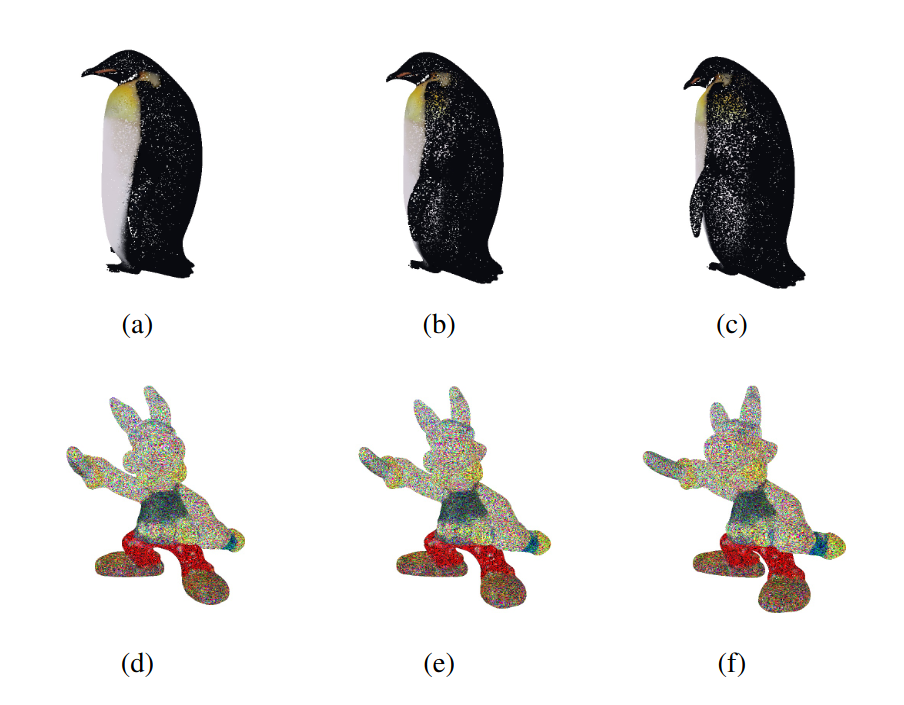
\includegraphics[width=0.75\textwidth]{imagenes/chapter4/ViewPoint}
  \end{center}
  \caption[Ejemplo de distorsiones que se presentan según la perspectiva]{
  Ejemplo de distorsiones que se presentan según la perspectiva.
Vemos que al girar el pingüino se empieza a observar un bajo número de puntos en su 
lateral izquierdo, permitiendo verse a través de él. De forma similar, 
en la imagen de abajo se ve cierta deformación de la cabeza.}
  \label{fig:ViewPoint}
\end{figure}

\begin{figure}
  \begin{center}
    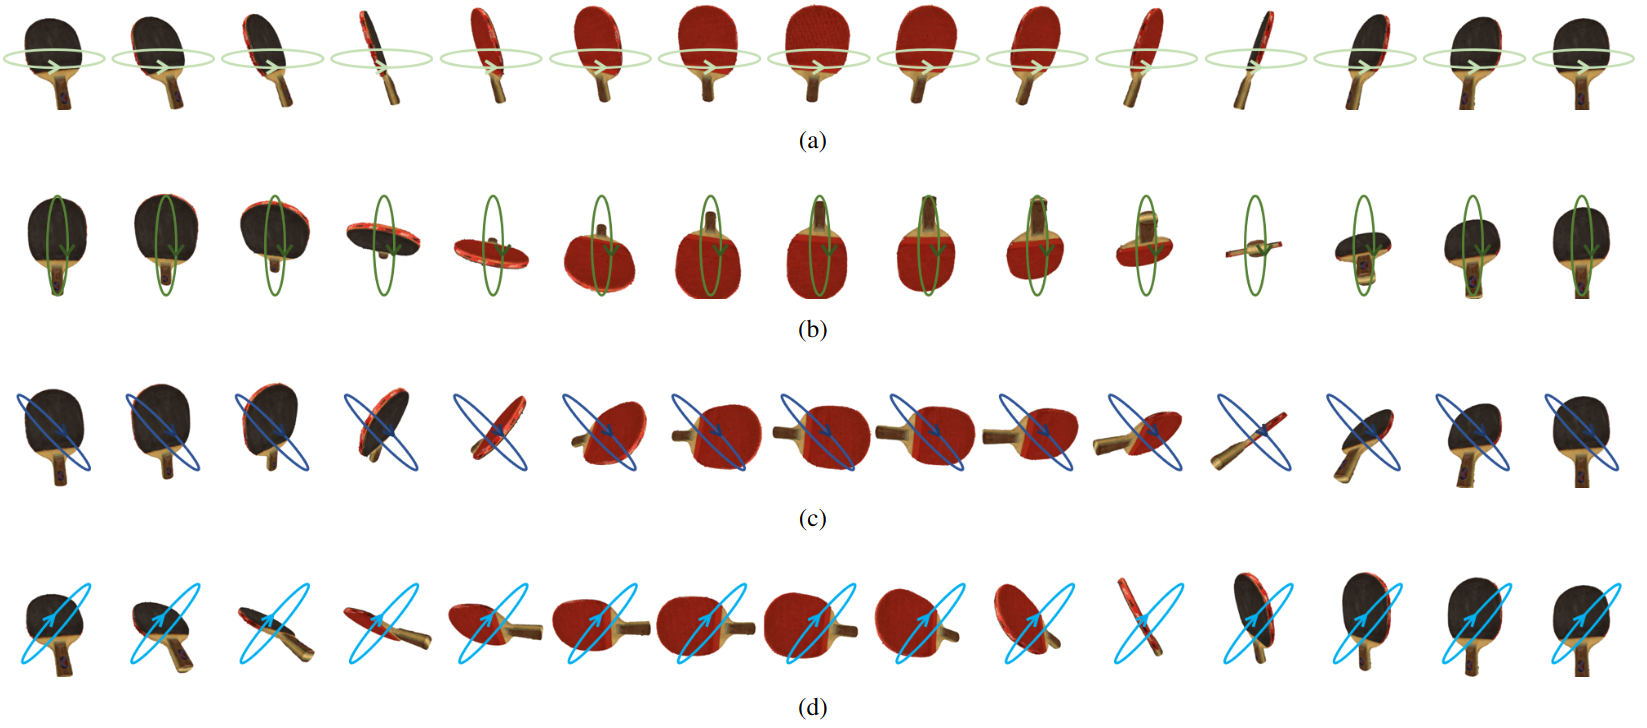
\includegraphics[width=\textwidth]{imagenes/chapter4/VQARotation}
  \end{center}
  \caption[Ejemplo de las rotaciones que utiliza el modelo VQA-PC\cite{VQA-PC}.]
  {Ejemplo de las rotaciones que utiliza el modelo VQA-PC\cite{VQA-PC}.
  Se observa que el final de cualquier eje de rotación es la posición inicial, 
permitiendo así unir de suavemente una secuencia de imágenes encadenada de los ejes 
que genere un video de rotación utilizado luego para la estimación.}
  \label{fig:VQARotation}
\end{figure}

Para realizar la secuencia de video, necesitamos realizar correctamente 
el conjunto de rotaciones descritos por las siguientes: 
\begin{equation}
  \theta_A = 
\begin{cases}
\begin{aligned}
   X_\alpha^2 + Y_\alpha^2 & = R^2 \\ 
    Z_\alpha & = 0 
\end{aligned}
\end{cases}
\label{eq:RotationA}
\end{equation}

\begin{equation}
  \theta_B = 
\begin{cases}
\begin{aligned}
   Y_\alpha^2 + Z_\alpha^2 & = R^2 \\ 
    X_\alpha & = 0 
\end{aligned}
\end{cases}
\label{eq:RotationB}
\end{equation}

\begin{equation}
  \theta_C = 
\begin{cases}
\begin{aligned}
   X_\alpha^2 + Y_\alpha^2 + Z_\alpha^2 & = R^2 \\ 
    X_\alpha + Z_\alpha & = 0 
\end{aligned}
\end{cases}
\label{eq:RotationC}
\end{equation}

\begin{equation}
  \theta_D = 
\begin{cases}
\begin{aligned}
   X_\alpha^2 + Y_\alpha^2 + Z_\alpha^2 & = R^2 \\ 
    X_\alpha - Z_\alpha & = 0 
\end{aligned}
\end{cases}
\label{eq:RotationD}
\end{equation}

Y para llevar a cabo la rotación debemos calcular el punto medio de la nube 
de puntos por medio de la siguiente ecuación \eqref{eq:PuntoMedio}:
\begin{equation}
  O_\sigma = \frac{1}{N}\sum_{n=1}^N \sigma_n
  \label{eq:PuntoMedio}
\end{equation}
Donde el $O_\sigma$ representa la coordenada (X,Y,Z) del centro medio de la 
nube de punto, y $\sigma_n$ representa la coordenada del punto $n$-ésimo punto. 
Utilizando ese centro, aplicamos las ecuaciones \eqref{eq:RotationA} a \eqref{eq:RotationD}.

Para extraer las características espaciales empleamos un modelo pre-entrenado, 
en concreto se investigó variaciones de esqueletos ResNet\cite{ResNet}. Una 
familia de redes residuales, que en su momento resolvieron el problema 
del estancamiento en el entrenamiento de redes neuronales profundas debido 
a la degradación del error. El único modelo al que optimizaremos sus pesos es 
ResNet, el modelo de extracción temporal solo es un paso previo.

\begin{figure}[htp]
  \begin{center}
    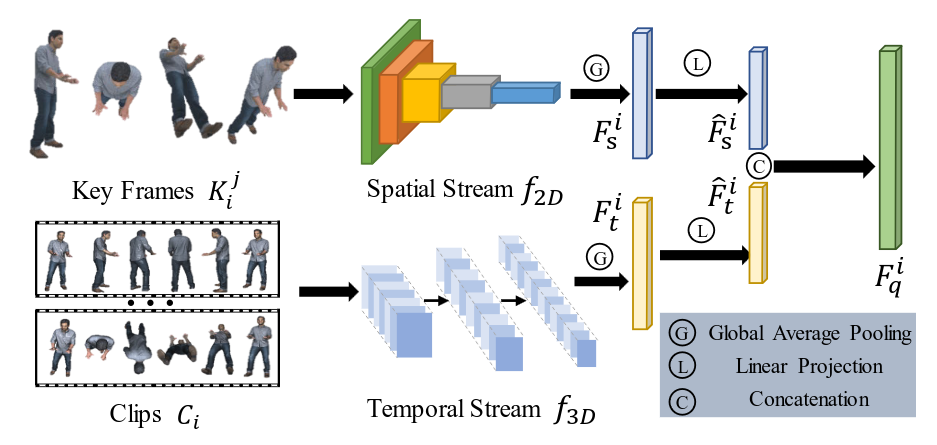
\includegraphics[width=0.70\textwidth]{imagenes/chapter4/PipelineCompleto}
  \end{center}
  \caption{Ejemplo detallado de las etapas del método de VQA-PC}
  \label{fig:VQAPipeline}
\end{figure}



